\chapter{Experiments}\label{experiments}
\section{HyperNEAT applied to the Ongoing Model}
Methodology vllt: Behavioud of ongoing and static model. TODO

\subsection{ES-EM learning}
\subsubsection{description}
To ensure that HyperNEAT works on this filed of application, a random connection sample was chosen. ES-EM connections were evolved by hyperNEAT all other connections were kept as randomly initiated. The aim of this experiment is to show that hyperNEAT can improve the moving behaviour of the arm by searching for an optimal ES-EM connectivity. That learning only the ES-EM connectivity is sufficient for to get an good behaviour was empirically proven by \cite{sebastianPaper}. (This experiment is parametrically equal to Nagel's ongoing experiment with $ppd =1, pa=1, w_e =\tau_{remaining/20}$. Note that those parameters haven't been explained here directly but they are identical with the way the Ongoing Model was explained in this work todo ref). Direct comparison between Nagel's and this experiment is not possible since here one pattern for all connections except of ES-EM were used while Nagel chose 100 different ones. 
The amount of neurons was set to 256 with the same type distribution explained in the methodology (TODO ref). Since the evaluation of the motor control model is computation expensive hyperNEAT searched only for an optimal solution to reach angles of 15\degree and 115\degree starting with an angle of 65\degree. Although training with more angles would be more promising, the basic concept of reacting to the critics input should be learned anyway. Further on the time to reach an angle was decreased from 120 to 40 seconds compared to Nagel to decrease the calculation time. This is justified because derived from the low rmsds of Nagels models couldn't needed much more than 20 seconds to reach their target angle. The fitness function $f_{ongoing}$ is given by:
\begin{equation}
	f_{ongoing}= 135-\dfrac{\sqrt{\frac{1}{40}\displaystyle\sum_{t=7}^{40} (\theta_t-15)^2}+\sqrt{\frac{1}{40}\displaystyle\sum_{t=7}^{40} (\theta_t-115)^2}}{2}
\end{equation} 
where $\theta_t$ is the forearms angel at time t. Both square root terms calculate the RMSD from a run from 7 to 40 seconds.( Note that this is the same scale than 20 to 120 seconds).(( Note that the time gap of 7 seconds is not necessary but makes the fitness more clear since the maximum value could theoretically be reached. 
450 generations were simulated and a population size of 90 were chosen.
Although 50 concurrent matlab instances were available a population size of 90 showed a better mean time performance for a individual than a population size of 100 or 80. Assuming an average calculation time of 8 minutes per generation (TODO real numbers) results in a calculation time of 60 hours. Whereby 40500 models have been evaluated.
The connection threshold $\theta_c$ is set to 0.8. The activation function of output neurons is set to a bipolar sigmoid function ($\frac{2}{1+\exp(-4.9x)}-1$) with a value domain of $[-1,1]$ next to $f(x)=2x$ on the x interval $[-0.4,0.4]$. If the output value of the sigmoid function is higher than 0.8 a connection is realized width the initial weight for this connection defined by the ongoing model. Note that weight scaling as usually done in HyperNEAT is not applied. Thus assuming the output of the sigmoid function is equal distributed between $-1$ and $1$  the threshold of $0.8$ leads to a connection realisation rate of $0.9$. (ncessary?). 
There are 4 types of activation function which a new node in the CPPN can get with equal probability. The available activation functions where bipolar sigmoid, Gaussian ($2\exp(-(2.5x)^2)-1 $), absolute value ($|x|$) and sine ($sin(2x)$). (TODO plot?) Which have been empirically proven to be successful for hyperNEAT experiments by \cite{HyperNeatMultiagent}. (at least for one todo)
Those are the base functions for the patterns created by CPPNS.
Based on the fact that cells of the brains sensory and motory cortex are aligned to each other along the approximately straight sulcus centralis, the cppn substrate configuration is chosen as two parallel lines of ES and EM neurons. The exact configuration can be seen in figure \ref{fig:ongoingsubstrate}.

\begin{figure}[tb]
	\centering
	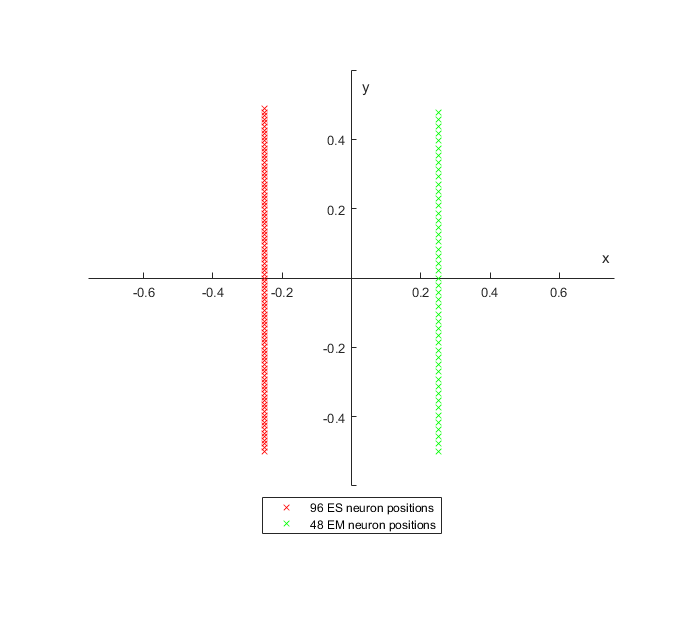
\includegraphics[width=0.7\linewidth]{figures/OngoingModel/OngoingSubstrate}
	\caption[Ongoing experiment substrate configuration]{\textbf{Ongoing experiment substrate configuration:} 96 Es neurons are placed with equal y distances between $(-0.25,-0.5)$ and $(-0.25,0.5)$. 48 EM Neurons are placed accordingly at $x=0.25$}
	\label{fig:ongoingsubstrate}
\end{figure}

The used NEAT parameters are as follows: A add connection mutation appears with a probability  of $0.15$, a add node mutation with $0.05$ and weight mutations with $0.96$ for each individual per generation. If a individual is selected to have a weight mutation depending on 5 equal probable metrics a varying amount of connections gets either assigned a randomly chosen new weight value or a even distributed value is added to the weight. The elitism proportion is $0.1$ which complies with 9 individuals. All CPPN connection weights were set to be in the interval $[-1.5,1.5]$.

To ensure that HyperNEAT gets the same fitness result when a model gets evaluated twice, the random number generation function is always initialized with the same seed. As a result HyperNEAT might now overfit during training, because the noise is always the same. Its fairly unlikely that Hyperneat can predict the random number generation function during simulation. So no benefit for the simulation is gained. Thus this is a simplification of Nagels Model that does no harm. TODO put in general description

TODO train and test data
TODO put neat params in general descriprion. 
TODO further on just give table with parameters.
\subsubsection{results}
The training  performance of the initial model with start angle 65\degree and target angle 15 and 115 \degree can be seen in figure \ref{fig:initialmodeltrain}. The behaviour at simulation of an angle of 35\degree are depicted in figure \ref{fig:initialmodelsim}. In training the initial model gets a fitness of $115.09$. The process of the HyperNEAT algorithm can be seen in figure (todo) and figure (todo). The first figure shows the mean fitness of each generation. The second the best fitness in each generation. And the third one the average complexity of each generation calculated by the total sum of nodes and connections of all individuals in this generation divided by the population size. 
As a representative set of models the 30 best models of HyperNEAt's last generation have been chosen. Since connection and node mutations are rare and most weight mutation in a CPPN have a minor influence on the behaviour of the model the best 30 models of previous generation behave similar. Thus it's irrelevant whether one analyses the best 30 models of the last generation or for example the 500 best models of all generations. TODO maybe in description
The ES-EM connection ratio of the initial model was $0.08$. HyperNEATs solution provide a higher ratio TODO  einfügen. As is shown in figure \ref{fig:connprobbox}. The RMSDs for reaching different angles are shown in figure \ref{fig:ongoingboxplot}.  The new models clearly outperform the initial one at reaching 135\degree. At the angles TODO new results. The behaviour of all 30 models reaching the angle of ... degree is shown in figure \ref{fig:meanmovement35deg}. And can be compared to the movement of the initial model in. figure \ref{fig:initialmodelsim}. The result of Nagel (figure \ref{fig:NagelOngoingBoxPlot}) show a lower RMSDs.  But the simulation results of this experiment are not fully comparable to Nagels result, since he used 500 randomly connected models. And this work only optimizes 1 randomly connected model with optimized ES-EM connections. But one can derive that an optimal ES-EM connection are not sufficient for optimal solutions(what was obvious anyway...;) ) (Thats more discussion).

TODO show best CPPN.  tell error of best model. argue that cppn not depictable but an example can be seen in model ...

 
\begin{figure}[tb]
	\centering
	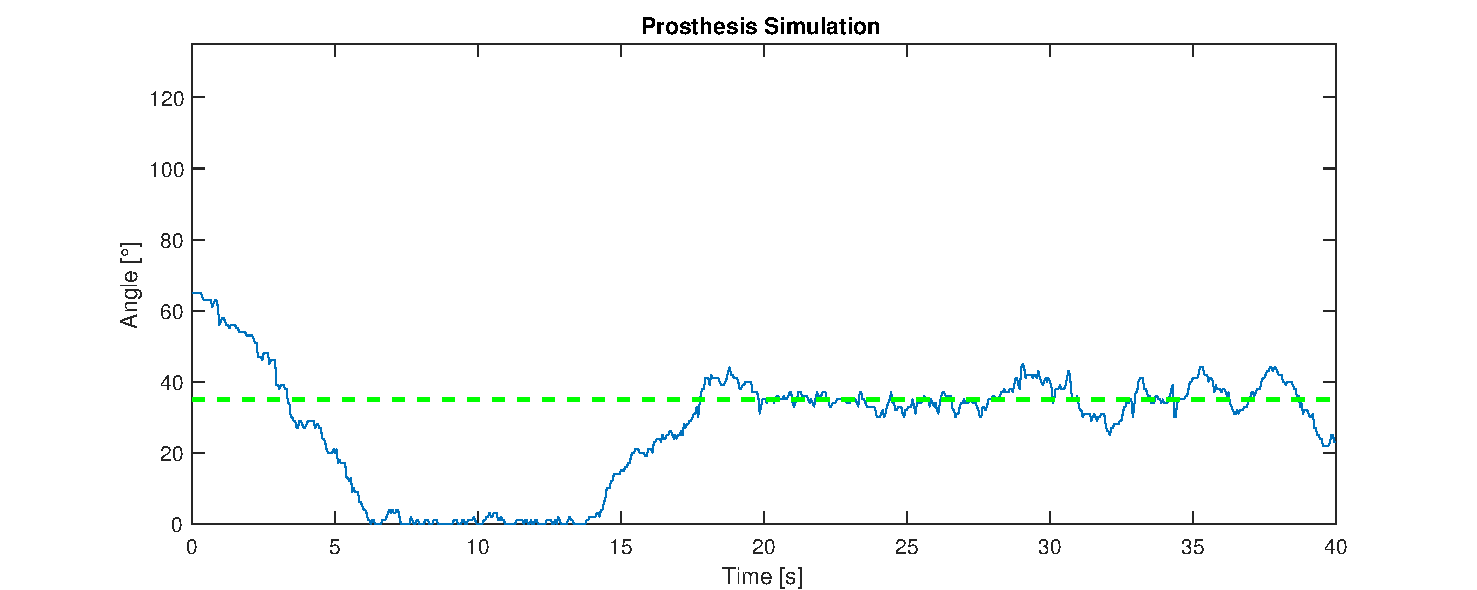
\includegraphics[width=0.7\linewidth]{figures/OngoingModel/InitialModelTrain-movement(start65-target35)RMSD=17,70511.pdf}
	\caption[Training behaviour of the initial ongoing model]{\textbf{Training behaviour of the initial ongoing model:} Sarting from 65\degree a 35\degree angle (blue) and 115\degree angle (red) is to be reached. The RMSD is 17.7\degree and calculated from 7 seconds onwards. }
	\label{fig:initialmodeltrain}
\end{figure}

\begin{figure}[tb]
	\centering
	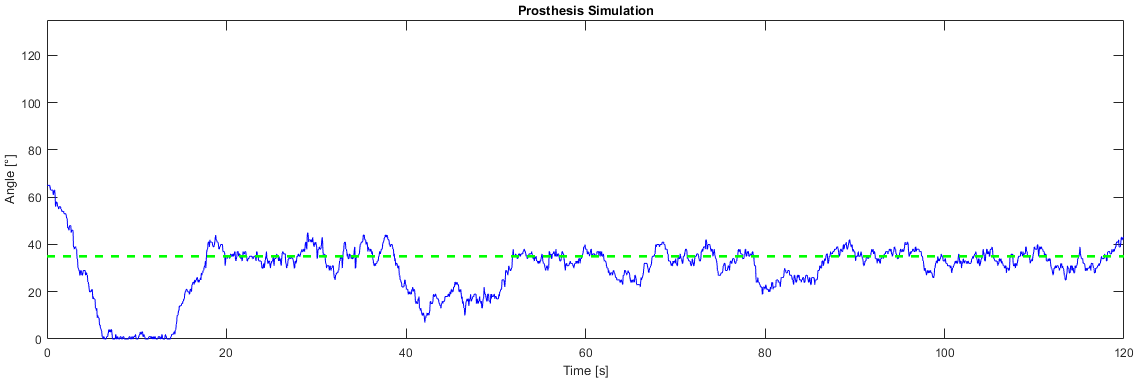
\includegraphics[width=0.7\linewidth]{figures/OngoingModel/InitialModelSim-movement(start65-target35)RMSD=7,56571}
	\caption[Simulation behaviour of the initial ongoing model]{\textbf{Simulation behaviour of the initial ongoing model:} Sarting from 65\degree a 35\degree angle is to be reached. The RMSD is 7.5\degree and calculated from 20 seconds onwards. }
	\label{fig:initialmodelsim}
\end{figure}



\begin{figure}[tb]
	\centering
	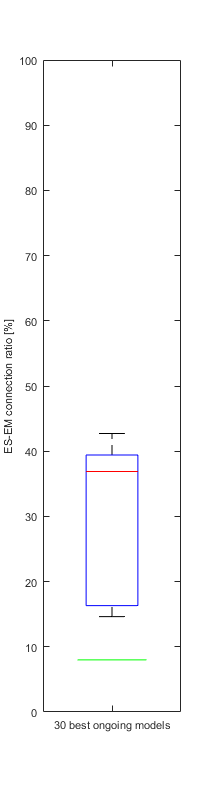
\includegraphics[width=0.7\linewidth]{figures/OngoingModel/connProbBox}
	\caption[Ongoing Experiment ES-EM connection ratios]{\textbf{Ongoing Experiment ES-EM connection ratios:} The connection ratio of the initial model is indicated by the green line.The mean of the 30 best ongoing model is represented by the red line. The box represents the interquartile range (IQR) from the first to the third quartile . The whiskers extend the quartiles by $\pm1.5\cdot IQR$. Red crosses show outlier.}
	\label{fig:connprobbox}
\end{figure}	

\begin{figure}[tb]
	\centering
	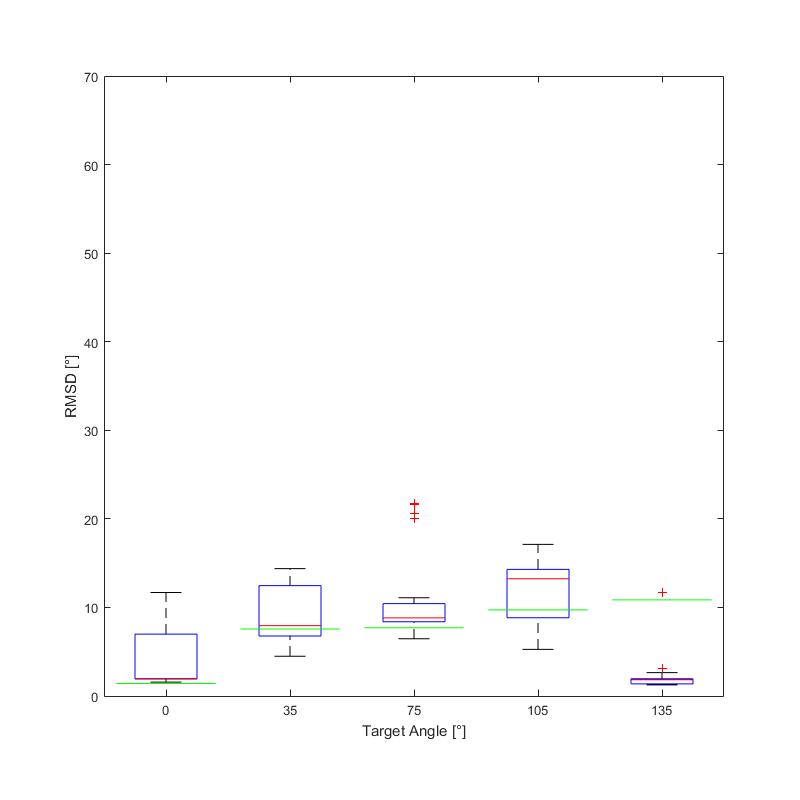
\includegraphics[width=0.7\linewidth]{figures/OngoingModel/ongoingBoxPlot}
	\caption[Ongoing Experiment RMSDS]{\textbf{Ongoing Experiment RMSDS:} The RMSD distribution of the 30 best ongoing models of HyperNEAT's last generation. Each Boxplot corresponds to one target angle: 0\degree, 35\degree, 75\degree, 105\degree and 135\degree. The initial angle was 65\degree. The RMSD of the initial model is indicated by the green line. The mean RMSD of the simulated models is represented by the red line. It is calculated from $t=20s$ until $t=120s$. The box represents the interquartile range (IQR) from the first to the third quartile. The whiskers extend the quartiles by $\pm1.5\cdot IQR$. Red crosses show outliers.}
	\label{fig:ongoingboxplot}
\end{figure}


\begin{figure}[tb]
	\centering
	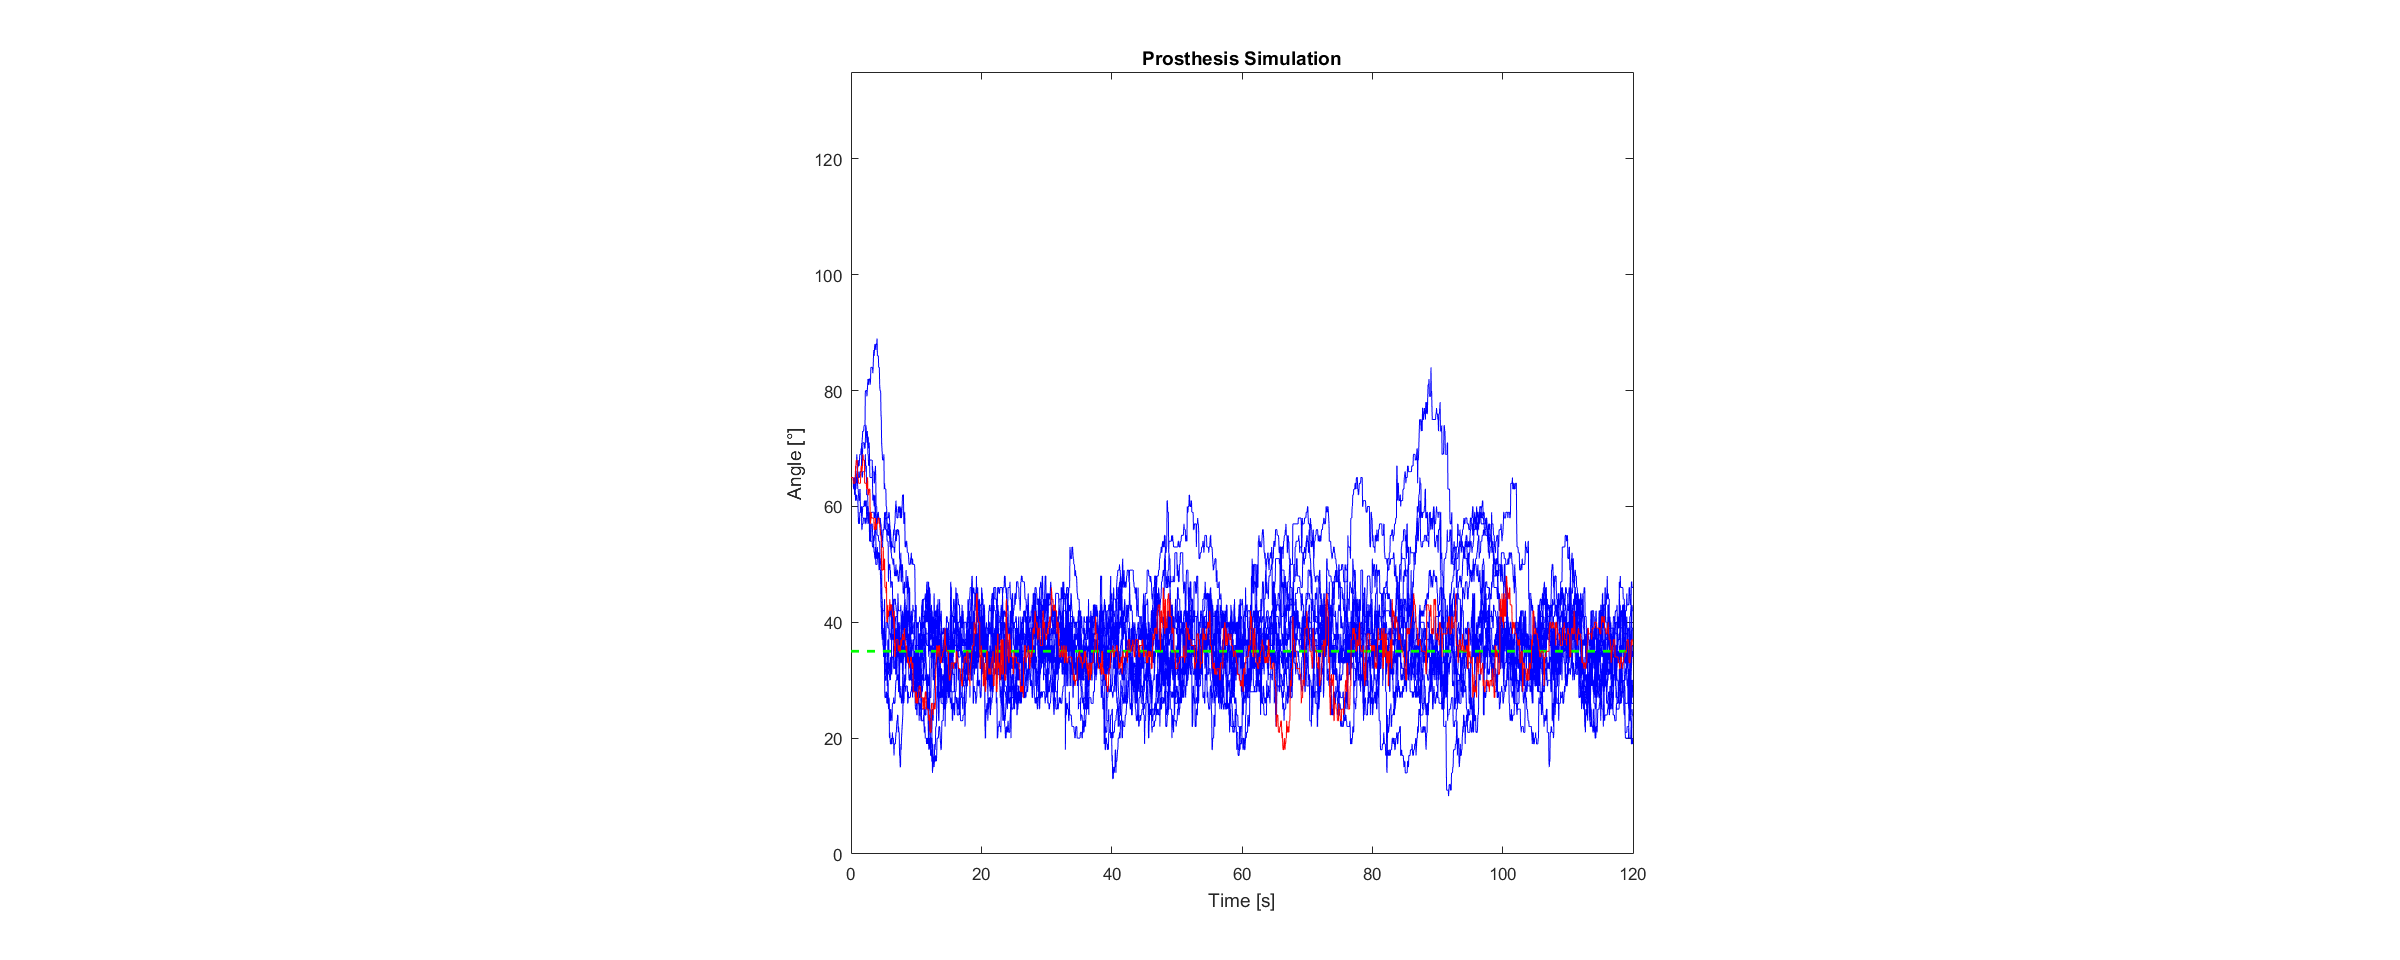
\includegraphics[width=0.7\linewidth]{figures/OngoingModel/meanMovement35deg}
	\caption[Ongoing Experiment mean movements]{\textbf{Ongoing Experiment mean movements:} The movements of the 30 best models of HyperNEAT's last generation are represented in blue. The red line is the mean movement. Form a start angle of 65\degree  the target angle of 35\degree was to be reached. The RMSD is ca 8 (todo calculate boxplot matlab mean)\degree and calculated from 20 seconds onwards. }
	\label{fig:meanmovement35deg}
\end{figure}

\begin{figure}[tb]
	\centering
	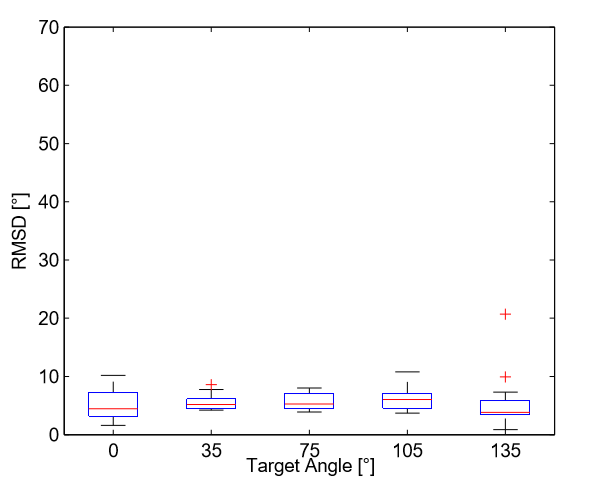
\includegraphics[width=0.7\linewidth]{figures/OngoingModel/NagelOngoingBoxPlot}
	\caption[Nagel's ongoing Experiment mean movements]{\textbf{Nagel's ongoing Experiment mean movements:} 100 models were generated. For each model 5 different target angles (0\degree, 35\degree, 75\degree, 105\degree 135\degree) were simulated in 5 runs per angle. The initial angle was 65\degree.  The mean RMSD of the simulated models is represented by the red line. It is calculated from $t=20s$ until $t=120s$. The box represents the interquartile range (IQR) from the first to the third quartile. The whiskers extend the quartiles by $\pm1.5\cdot IQR$. Red crosses show outliers. \cite{sebastianMasterThesis} }
	\label{fig:NagelOngoingBoxPlot}
\end{figure}

\subsubsection{discussion}
TODO
\section{HyperNEAT applied to the Static Model}
-> methodology 304 neurone bei statischem lernen

-learning: min max angle to be reached
-> average time for learning phase 79 seconds.  | i am better
-> shortest 19.6 seconds.
-> longest 1249 seconds.
SSP used | i not
same eligibility time windows,
same amount of cells
same cells fireing per angle .
tau learning is dynamic.

-my fitness function
	argue that rmsd over whole movement not after reached is calculated.
	
- boxplot time to complete learning phase. (change matlab code)
- RMSDs for each target angle box plot.
- boxplot total rmsd.

simulation:
RMSD calculated the last 20 second of 30 seconds time window!
-> but still argue that my model would have a lower total rmsd.
 
 -> how long does the best model need to reach each angle in average. (sebastian 35)
     -> how much better to chadderdon( sebastian 85 prozent besser)
     
 argue as sebastian did that only movement is learned directly resting not. ok( actually it is). But no resting mechanism in netowrk,


\subsection{D-ES learning}
min variance experiment. 
            rmsd_scale=0.7;
angle_scale=0.2;
training_scale =0.1;
%Static_RMSDFit_17_07_10_minVariance.txt Threshold= 0.3 rate= 0.6914 meanFitness= 0.85 approxRmsd = 28.66


-> one model optimized. Check baseline model again.
-> Hyperneat performance
-> CPPN
-> best model
-> box plot compares.


\subsubsection{description}
\subsubsection{results}
\subsubsection{discussion}
\subsection{All Connections 2D neuron space}
\subsubsection{description}
\subsubsection{results}
\subsubsection{discussion}
\subsection{All Connections 1D neuron space}
\subsubsection{description}
\subsubsection{results}
\subsubsection{discussion}

\section{ES-HyperNEAT applied to the Static Model}
\subsection{All Connections and Neurons 2D neuron space}

\subsubsection{description}
\subsubsection{results}
\subsubsection{discussion}

\subsection{All Connections and Neurons 1D neuron space}

\subsubsection{description}
\subsubsection{result}
\subsubsection{discussion}